
\section{くまのまつり ― 地域と共に創るお祭り}
\label{sec:kumanomaturi}

\subsection{くまのまつりとは}

熊野寮では, 5月, 8月, 11月に「くまのまつり」というお祭を開催しています. このお祭は, もともとは地域の商店の方々が2010年に立ち上げ, 翌年から寮自治会との共催で開いているものです. これは地域と一緒につくるお祭りであり, 寮自治会としては寮外との連帯を目指すためのお祭です.

お祭では地域の飲食店や雑貨店, 個人など30組以上の外部出店ブースが並びます. ステージパフォーマンスや子供向けの企画もあり, とにかく楽しいお祭です. 来場者は2日で2000人にも及びます. Facebook「くまのまつり」ページにも写真がたくさん載っているので見てみてください.

\subsection{くまのまつりを行う意味}

ここでは「くまのまつり」開催の意義を少し掘り下げます. 端的に言えば, 「熊野寮の素晴らしさを外部に発信する場」として「くまのまつり」があります.

現政権の方針に従って動く公安警察や京大当局は, 熊野寮に対して激しいネガティブキャンペーンを張ってきました。


まず、2013年から毎年のように, 公安警察による熊野寮の家宅捜索が行われています. 2014年からはそれが大々的に全国に報じられるようになり, 寮生も度々逮捕されるようになりました. 家宅捜索の中で公安警察が行う違法行為・人権侵害に対して激しく抗議することもあります.  一部の報道によって「過激派の巣窟」というイメージを持っている方もいるでしょう.

そもそも私たちは議論によって, 学生による寮の自主管理・運営を行っています. これは, ともすれば住人のエゴによる運営に成り下がってしまうものです. しかし, 私たちはエゴではなく, 「京大で学ぶ者に福利厚生を提供する」という熊野寮の役割を果たし, さらにより良い福利厚生のあり方を追求するために議論し, 寮自治会としての行動をとっています. さらに言えば, 教育を受ける権利を保障するための熊野寮は社会的にも必要なものであり, 我々寮自治会の活動は社会的にも必要なものだという自負があるのです.

例えば, 公安警察に対する激しい抗議には「住んでいる学生の生活と権利を守るため」という意義があります. 安心して暮らせる住居としての熊野寮を守るための行動です. しかし, この行動も「過激派の巣窟」を描く材料にされてしまいます.


\begin{figure}[H]
  \centering
  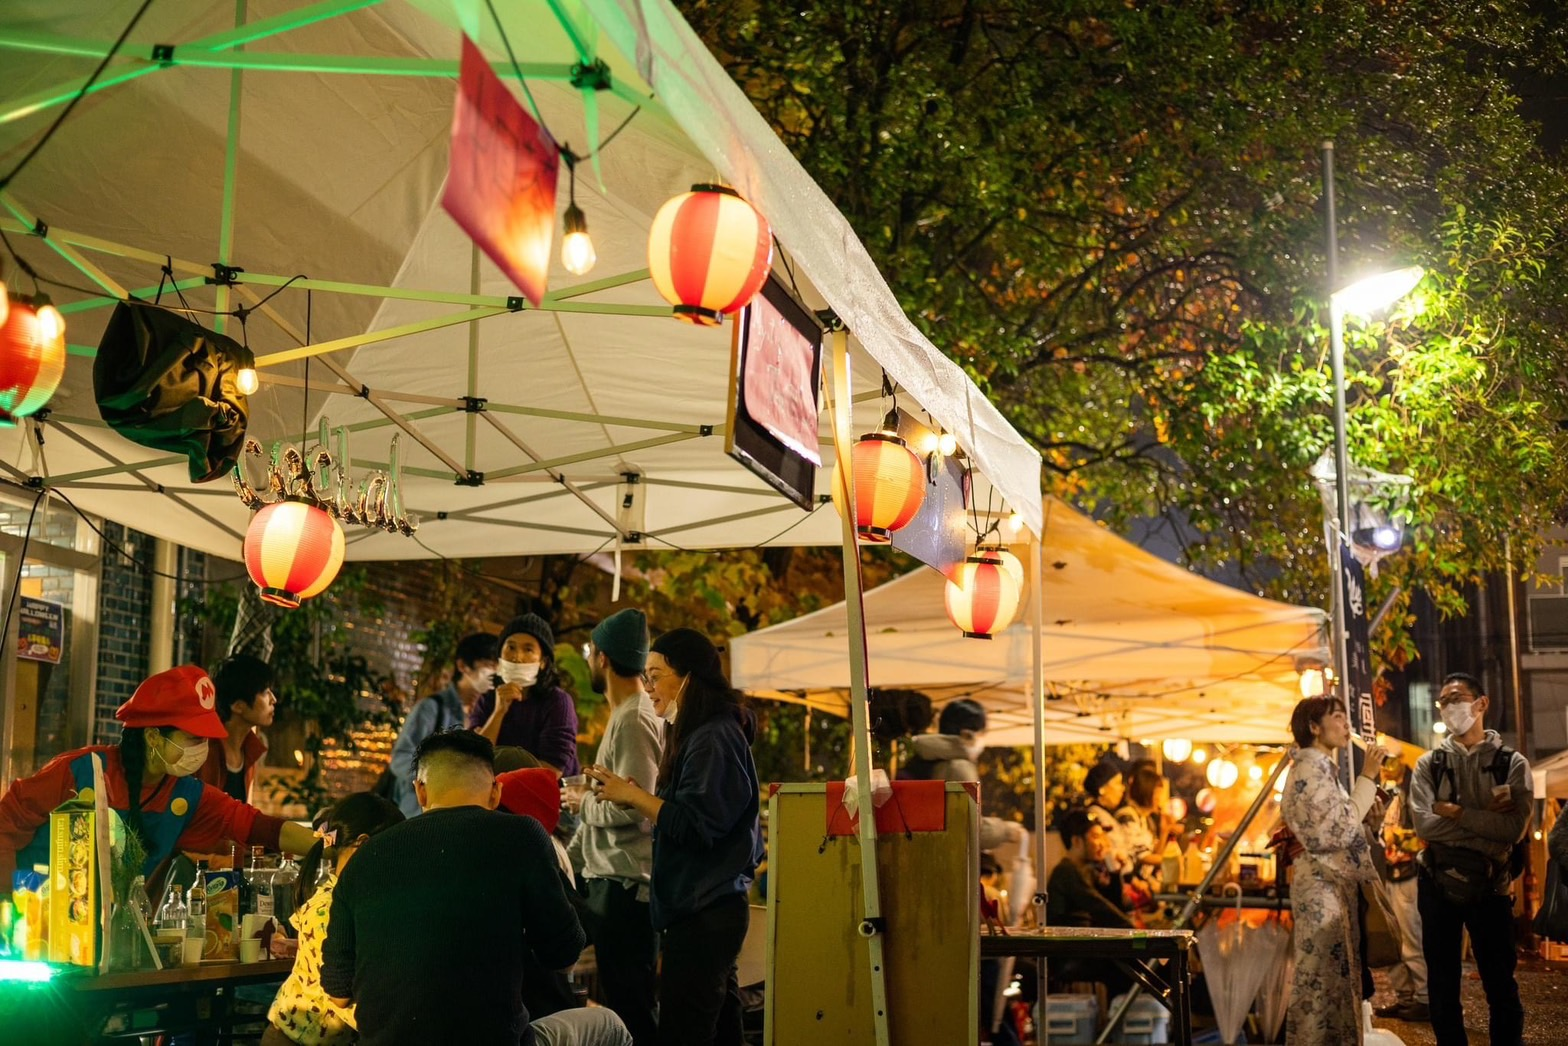
\includegraphics[width=10cm]{gazo/kumanomaturi1.jpg}
\end{figure}

さて, そこで私たちがお祭りを通してアピールするのは「過激派の巣窟なんかじゃありません」ということなのか. それは違います.空虚で中身のないレッテル貼りに対して単に「違います」「住んでいるのは普通の学生が殆どです」などと“健全さ”をアピールするのもまた空虚でしょう. 寮生が何を考え, 寮自治会がどういう理念をもってその活動を展開しているのか, 見えにくい中身の話を対面で真摯に説明することにこそ意味があります.

大事なのは, 真っ当な内容が伴っているかということだと思います. 「学ぶ権利を守るためにここまでやります」と丁寧に説明した上で, 「団体交渉を要求するとか, 昔の学生運動みたいで過激だね」と言う方もいらっしゃいますが, 理解した上で「過激だ」と言うのは当人の自由でしょう.

レッテル貼りの材料にされようとも, 過激に見えるかもしれない抗議を続け, 中核派の学生の人権を守る,そういった中には「誰でも安心して暮らせる住居を守る」「寮を必要とする学生には住居を保障する」という, 寮自治会が貫くべき理念があります.そして,実際に祭りで説明を聞いてくださった多くの地域住民が, 警察や京大当局による一方的な権力行使に対して批判する立場に立ってくれています.

ともすれば誤解されてしまう, しかし本当は非常に重要な寮自治会の内実を, しっかりと社会に発信し, 地域の方々と顔の見える関係をつくる中で広げていこうというのが「くまのまつり」の取り組みです.

今でこそ, 盛大なお祭になった「くまのまつり」ですが, はじめからそうだったわけではありません. 寮生や寮外の協力者がお店や知人に呼びかける中で, 毎年少しずつ輪が広がっていき, このような盛大なお祭へと成長していきました. やりたいと思ったことを何でも実行に移せるのが自治寮のいいところです. 「くまのまつり」は自治会のもつ無限の可能性の一つを示す取り組みです. 入寮を検討される皆さんには入寮してもしなくてもぜひ「くまのまつり」に遊びに来てほしいと思います. 入寮してもしなくても是非一緒にお祭りやりましょう!

皆でアイデアを出し合いながらお祭を創りあげていく過程, ご近所の人と出会い語る中で新たな関係を創りあげていく過程では, かけがえのない団結が生まれます. それが熊野寮をよりよい自治寮に変えていく何よりのエネルギーなのです.




\begin{figure}[H]
  \begin{minipage}[H]{.5\textwidth}
    \centering
    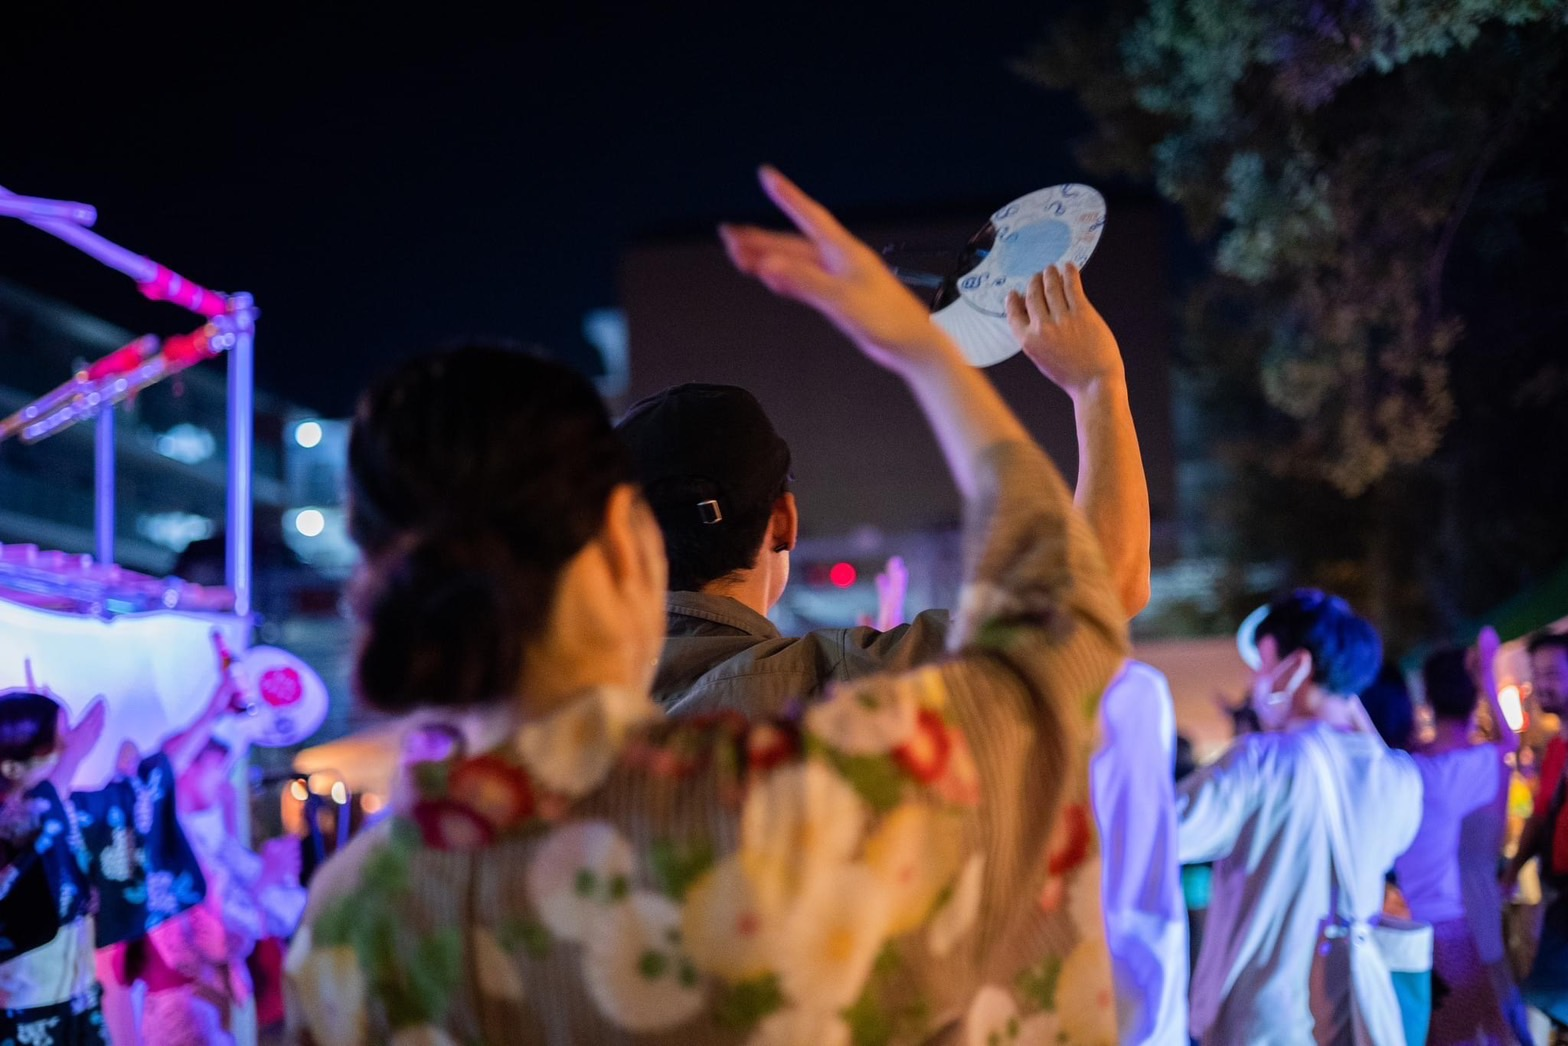
\includegraphics[width=8cm]{gazo/kumanomaturi2.jpg}
  \end{minipage}
  \begin{minipage}[H]{.5\textwidth}
    \centering
    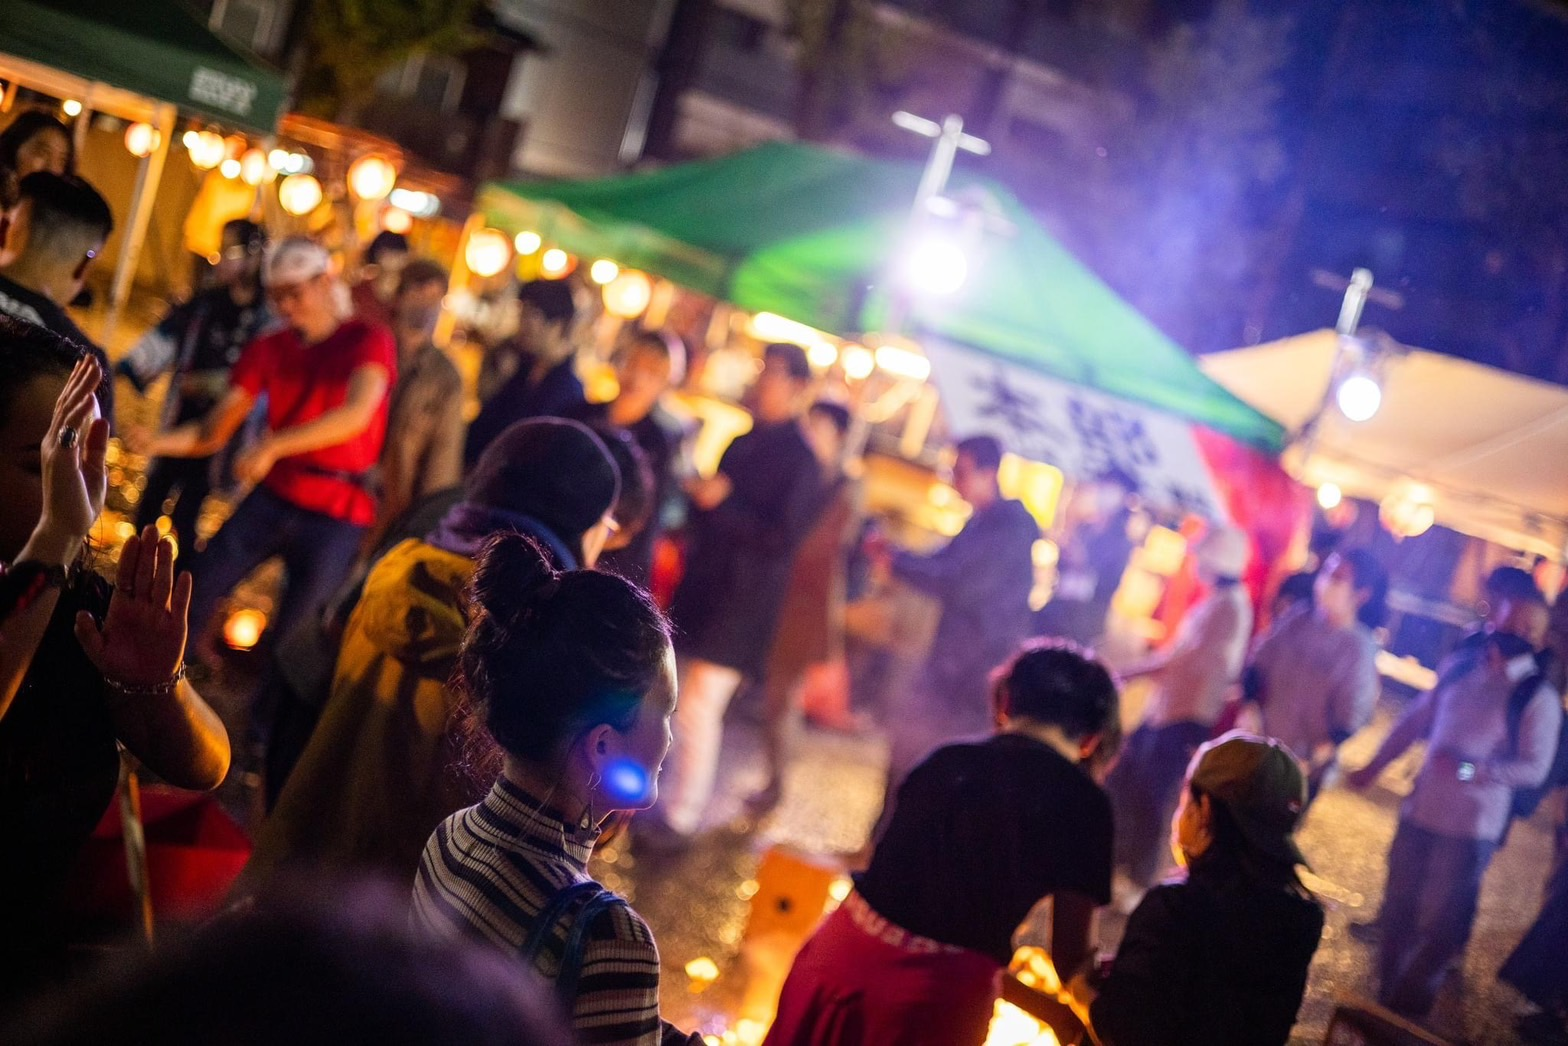
\includegraphics[width=8cm]{gazo/kumanomaturi3.jpg}
  \end{minipage}
\end{figure}

